\section{Introduction/Overview info}
\begin{itemize}
    \item The LHC is the largest single machine in the world. It's the largest machine ever constructed by humans.
    \item Note about how the LHC enables ATLAS physics, is a unique laboratory environment, and a towering achievement of humankind.
    \item Grateful for people's effort in building such a large machine.
    \item Building the LHC is not just an impressive feat in absolute terms, it is also impressive compared to humanity's other accelerators. Three other large superconducting accelerators: Tevatron, HERA, RHIC use Nb-Ti superconductor, at about 4.2K, and fields around 5 T. How to increase to 8 T? \cite{lyndon}
    \item Technical facts to illustrate this challenge.
    \begin{itemize}
        \item 26.7 km circumference
        \item SPS injects at 450 GeV \cite{lyndon}
        \item Designed luminosity $1.0\times10^{34}cm^{-2}s^{-1}$ \cite{lyndon}
        \item Designed energy 14 TeV \cite{lyndon}
        \item It takes 15 days to cool or warm a sector. This can be speed up using two cooling stations \cite{lyndon}
        \item LHC is first hadron machine with non-negligible synchrotron radiation. Influenced design of cryo and vacuum systems \cite{lyndon}
    \end{itemize}
    \item LHC is built from subsystems: magnets, vacuum, cryogenics, RF, power, injection, extraction, beam instrumentation, collimation, controls. \cite{lyndon} These will be described here.
    \item LHC is a machine under continuous development. The only place to improve the LHC is at the LHC. Therefore will discuss the history of LHC in final section.
\end{itemize}

\section{Civil Engineering}
\begin{center}
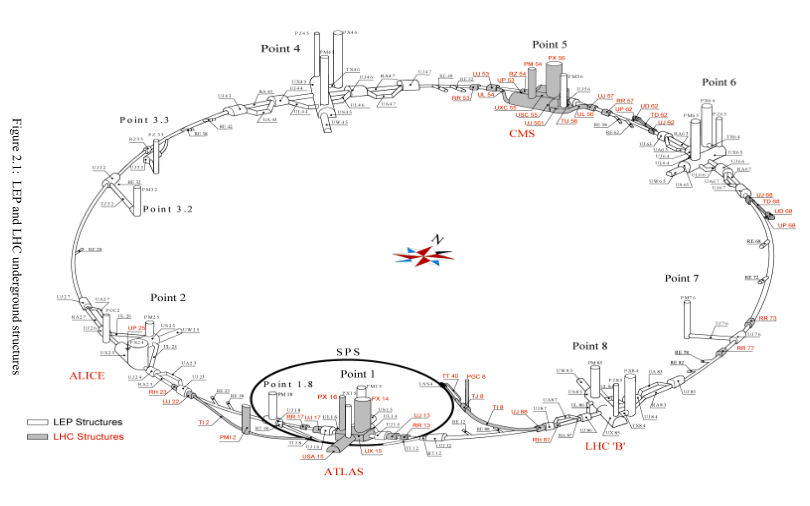
\includegraphics[width=0.5\textwidth]{figures/notes-experiment/lhcLepLayout.png}
\end{center}
\begin{itemize}
    \item Before building the accelerator, civil infrastructure is needed
    \item The Tevatron is buried less than 10m deep, which could be accomplished by cut-and-fill. RHIC is primarily above ground. Neither approach was suitable for the original LEP tunnel. 
    \item A different approach was needed for LEP based on the area's \textbf{geology}:
    \begin{itemize}\scriptsize
        \item Land here is layer of moraine (unconsolidated loose rock) over molasse (soft sediment, sometimes contains ground water). \cite{lhcDesignV2}
        \item 23km of tunnel in Lemanic basin molasse. This is Cenozoic and formed from marine deposites. \cite{lhcDesignV2}
        \item The Jura side is Mesozoic, limestone \cite{lhcDesignV2}
    \end{itemize}
    \item LEP was buried 45-170m, so a cut-and-fill approach was not possible.
    \item Beginning in 1985, the tunnel was mostly dug with three tunnel bores. When the molasse was unsuitable explosives were used.
    \item CERN has a long history of building accelerator and civil infrastructure. The design of the LHC leveraged this to reduce costs.
    \item Every LEP building has been reused for the LHC. Much of the civil infrastructure was reused as well. What was already built from LEP:
    \begin{itemize}\scriptsize
        \item \textbf{physical details:}
        \item Tunnel diameter 3.8 m, too small to hold separate rings \cite{lyndon}
        \item Tunnel depth 45-170m. 1.42\% slope towards the lake. The slope avoids a deep moraine near airport \cite{lhcDesignV2}
        \item Tunnel has 8 arcs, 8 straight sections of approx 528m length. \cite{lyndon}
        \begin{itemize}\scriptsize
            \item 4 straight sections for experiments \cite{lyndon}
            \item others used for RF, collimation, abort, utilities \cite{lyndon}
            \item ATLAS at p1 \cite{lyndon}
            \item CMS and TOTEM at p5 \cite{lyndon}
            \item ALICE p2 \cite{lyndon}
            \item LHCb p8 \cite{lyndon}
            \item Injection at p2 and p8 \cite{lyndon}
            \item Collimation at p3, p7 straight sections. p3 momentum collimation, p7 beam halo (betatron) \cite{lyndon}
            \item p4 has RF , one for each beam, operating at 2x injection frequency (RF is 400Hz) \cite{lyndon}
            \item p6 has abort systems, extract beam and dump into absorbers \cite{lyndon}
        \end{itemize}
    \end{itemize}
    \item Additional infrastructure was required for the LHC.
    \begin{itemize}\scriptsize
        \item Major expansion of tunnels: mostly for new injection lines, and beam dumps. \cite{lhcDesignV2}
        \item Additional new caverns needed for ATLAS and CMS (ALICE and LHCb reuse existing caverns). Each has two main caverns. \cite{lhcDesignV2}
        \item Two new injection tunnels leading from SPS, with internal diameter 3.76m, excavated diameter 4.5m. The length of each is approx 2.5km. \cite{lhcDesignV2}
        \item LEP flooded on two occasions. To avoid, steps including additional draining. Water is pumped to the surface. \cite{lhcDesignV2}
        \item For CMS, the moraine layer is thicker, and a freezing technique was used. Not use for ATLAS \cite{lhcDesignV2}
    \end{itemize}
    \item Building process timeline:
    \begin{itemize}\scriptsize
        \item Civil engineering lasted 5 years, except CMS which took 6.5. \cite{lhcDesignV2}
        \item P1 work began April 1998 \cite{lhcDesignV2}
        \item In addition to existing buildings, 8 new building built at P1. \cite{lhcDesignV2}
        \item P1 has 2 new shafts over experimental cavern, 1 over each service cavern. \cite{lhcDesignV2}
    \end{itemize}
\end{itemize}

\section{Machine Layout}
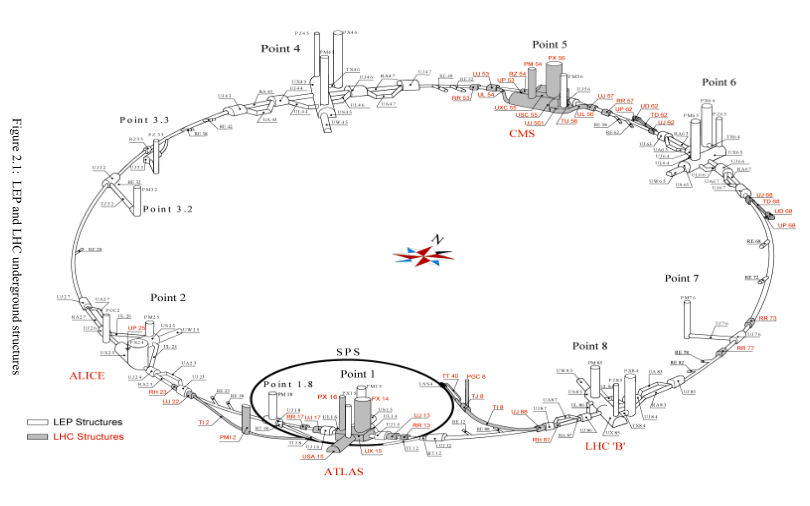
\includegraphics[width=0.5\textwidth]{figures/notes-experiment/lhcLepLayout.png}
\begin{itemize}
    \item Built in tunnel, on the outer side of the tunnel.
    \item Not completely circular, instead there are 4 straight sections, and 4 curved sections. \cite{lyndon}
    \item Experiments, RF, collimation, abort/beamdump, utilities, and services are located in straight sections \cite{lyndon}
    \begin{enumerate}\scriptsize
        \item p1: ATLAS
        \item p2: ALICE, clockwise injection
        \item p3: Momentum collimation
        \item p4: RF, one for each beam
        \item p5: CMS and TOTEM
        \item p6: Abort systems to extract beam and dump into absorbers
        \item p7: beam halo (betatron) {\color{blue} ???}
        \item p8: LHCb
    \end{enumerate}
\end{itemize}

\section{Accelerator Design}
\begin{itemize}
    \item The heart of the LHC is the accelerator.
    \item Acceleration takes place only in a short section of p4
    \item The circular design of the LHC means beams repeatedly through the same accelerator, so not much acceleration is needed per turn.
    \item For hadrons, not much energy is lost in a revolution from synchrotron radiation, so the accelerator segment only needs to exceed the energy lost.
    \item Synchrotron beam radiation loss is only 3.7 kW/beam (in planned operation, lumi). Each cavity provides 32kW to increase the beam energy. The RF power is not determined by beam power, but by the required RF voltage. \cite{boussard}
    \item The principle behind the LHC acceleration is RF cavities, described earlier.
    \item Independent systems for individual control of beams \cite{lyndon}
    \item Physical description of cavities
    \begin{itemize}\scriptsize
        \item Cavities are copper, sputtered with niobium(vapor deposition technique, ``microscopic particles of a solid material are ejected from its surface, after the material is itself bombarded by energetic particles of a plasma or gas''). {\color{blue} From \url{https://accelconf.web.cern.ch/SRF91/papers/srf91e11.pdf}, better than solid niobium for thermal conductivity. Niobium is superconductive, so better RF performance. Also, is cheaper to use super thin layer.} \cite{lyndon}
        \item Choice for superconducting: high field, small machine impedance, high stored energy. {\color{blue} Not clear yet what means} \cite{boussard}
        \item Operating temp 4.5 k, each cryomodule has its own helium tank. \cite{boussard}
        \item The phase modulation $\delta\phi$ has max value: $\delta\phi\le0.5(R/Q)\omega_0(I_b/V)\tau$, for gap length $\tau$. $R/Q$ si geometric cavity parameter, $\omega_0/2\pi$ is RF frequency, $I_b$ is RF from beam current, V is cavity voltage. Phase modulation $\delta\phi$ leads to IP displacement. The superconductive cavities allow the R/Q to be smaller. Q may be \emph{quality factor} or peak energy / energy lost per cycle. R may be resistance across the cavity, but am unsure. \cite{boussard}
        \item R/Q = $44\Omega$, 2MV/cell, 11.8MV/m.  \cite{boussard}
        \item Sputtered by magneton sputtering, 1-2 microns thick  \cite{boussard}
        \item The caveties can be mechanically distorted by tuners. Tuner is used to compensate beamloading {\color{blue} inaccuracy? Arrival time?} \cite{boussard}
    \end{itemize}
    \item Physical description of groups of cavities
    \begin{itemize}\scriptsize
        \item Eight single cell cavities per beam, each 2 MV (5.3 MV/m. Frequency 400 MHz. Total is 16MV per beam. \cite{boussard}
    \end{itemize}
    \item Powering the cavities
    \begin{itemize}\scriptsize
        \item RF power is supplied to the cavities by a variable power coupler. This consists of a waveguide of adjustable length. Adjusting the length modifies the cavities external Q factor. A voltageof 3kV is applied to the antenna to reduce multipactor (electron avalanche). \cite{boussard}
        \item Cavities have two couplers attached, one of which coupler is connected to 500 kW 400MHz klystron. The other is attached to a resistive load. {\color{blue} Should check current config, this was a test} \cite{boussard}
        \item One klystron per cavity, which needs to be capable of supplying 200kW. \cite{boussard}
    \end{itemize}
    \item Before manufacturing, a prototype with 2 cavities was built. Also tested was cryostat \cite{boussard} \\
    \begin{center}
        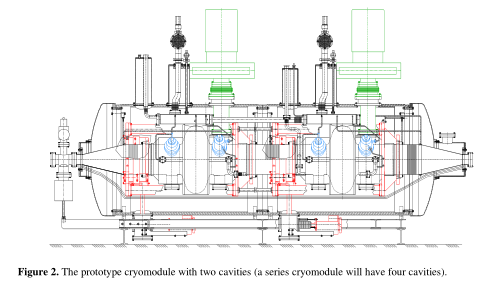
\includegraphics[width=1\textwidth]{figures/notes-experiment/rfproto.png}
    \end{center}
\end{itemize}

\section{Magnet Design}
\begin{itemize}
    \item If the accelerator is the heart of the LHC, the magnets are the body of the LHC.
    % ####################
    % Description of all magnets
    % ####################
    \item Magnets serve multiple purposes \cite{lyndon}
    \begin{itemize}\scriptsize
        \item Dipole magnets to bend the beam around the curved sections. There are 1232 main dipoles
        \item Quadrupole magnets to focus and defocus the beam. Each quadrupole simultaneously focuses in one direction and defocuses in an orthogonal direction. There are 392 arc quadrupoles throughout the LHC.
        \item Sextupole for correcting chromaticity introduced by quadrupoles, there are 2464
        \item Other magnets such as octupole and decapole correctors fill in the remaining 7000 superconducting magnets.
    \end{itemize}
    \begin{center}
        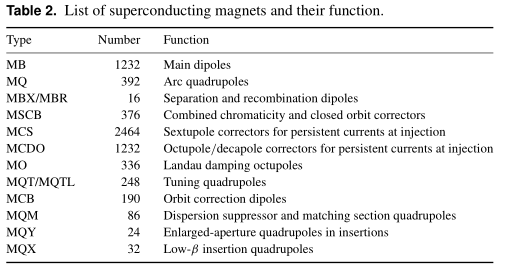
\includegraphics[width=0.6\textwidth]{figures/notes-experiment/listmagnets.png}
    \end{center}
    % ####################
    % Description of dipole
    % ####################
    \item The job of bending the beam around the LHC is performed by the dipole magnets.
    \begin{itemize}\scriptsize
        \item b-field of dipoles is 8.3 T \cite{lyndon}
        \item Superconducting material is NbTi \cite{lyndon}
        \item Two sets of magnet coils in common yoke and cryostat \cite{lyndon}
        \item Dipole length 14.2m of magnet, 15m total. Dipoles wired in series. \cite{lyndon}
        \item Coils held in austenitic (non-magnetic, stainless steel, low permeability steel) steel collar, surrounded by a yoke of low carbon steel to carry magnetic flux. Field: \cite{lyndon}
        \begin{center}
            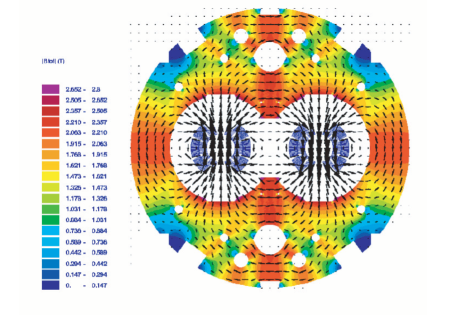
\includegraphics[width=0.5\textwidth]{figures/notes-experiment/field.png}
        \end{center}
        \item Coils wound in two layers, in 6 blocks. Copper wedges separate. Optimized to keep pure dipole field. \cite{lyndon}
        \begin{center}
            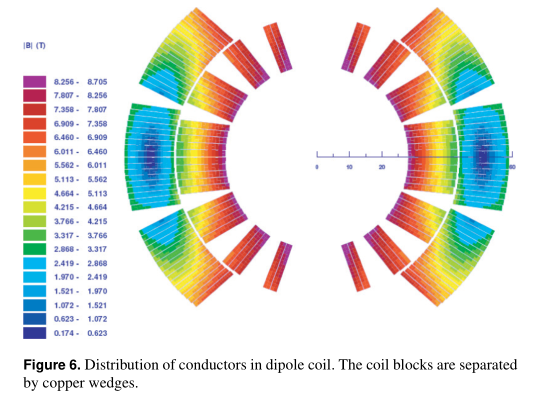
\includegraphics[width=0.5\textwidth]{figures/notes-experiment/coils.png}
        \end{center}
    \end{itemize}
    % ####################
    % Magnet periods
    % ####################
    \item Magnets are grouped in periods. Each period (identical focusing properties) is 106.9m long, and has 6 dipoles, and 2 6.6m \emph{short straight sections} (SSS) that contain quadrupoles and lattice correctors. \cite{lyndon}
    \item Each SSS also contain sextupoles for chromaticity control, and orbit correction dipoles. Also sometimes contain octupoles or trim/skew quadrupoles. \cite{lyndon}
    % ####################
    % After finishing arc
    % ####################
    \item After arc, ``dispersion suppressor'': adapts orbit to shape of tunnel, cancel horizontal dispersion from the arc, match beams between the arcs and straight sections. {\color{blue} See notes in next section \url{https://accelconf.web.cern.ch/p79/PDF/PAC1979_3493.PDF}} \cite{lyndon}
    % ####################
    % Cryo system
    % ####################
    \item Supporting the magnets is an elaborate cryosystem
    \begin{itemize}\scriptsize
        \item Three other large superconducting accelerators: Tevatron, HERA, RHIC use Nb-Ti superconductor, at about 4.2K, and fields around 5 T. How to increase to 8 T? \cite{lyndon}
        \item Considered Nb3Sn, but this is brittle and needs to be heated for many hours at 600 degrees \cite{lyndon}
        \item 1.8K NbTi has about 10\% heat capacity than it does at 4.5K, meaning it can heat faster and quench more \cite{lyndon}
        \item Cryo system in run 1 was most faulty, followed by injector systems. 25-30\% of fault time. \cite{lhcRun1}
        \item Dipoles operation 1.9 K superfluid helium. Total 100 tons. Helium's phase transition at 2.17k to become superfluid \cite{lyndon}
        \item LHC is first hadron machine with non-negligible synchrotron radiation. Influenced design of cryo and vacuum systems due to heat load \cite{lyndon}
        \item \textbf{Quench protection:} if a quench is detected, capacity bank is ``fired'' into the coil to make it resistive. The current is diverted through a diode. Then the power is shut off. \cite{lyndon}
        \item \textbf{Cryo. System} Superfluid helium's low viscosity allows it to permeate coil insulation, and directly cool superconductor. This also increases the specific heat of the system, as its specific heat is 2000 times that of the superconductor. It effectively transports heat out. \cite{lyndon}
        \item Magnets are surrounded by 1bar LHe, and a pressurized 15mbar pipe of LHe is pumped past as a heat exchanger. This keeps the LHe in the coil permanently liquid - no vapor \cite{lyndon}
        \item It takes 15 days to cool or warm a sector. This can be speed up using two cooling stations \cite{lyndon}
        \item When planning the required quality of LHC magnets, simulations were run with random and systematic magnet imperfections. The requirement was the for the ``dynamic aperture'' of the beam to be 6sigma smaller than the beam pipe after 10e6 turns (several minutes) \cite{lyndon}
    \end{itemize}
\end{itemize}

\begin{itemize}
    \item Amplitude function $\beta$ may be transverse beam size? \cite{boussard}
\end{itemize}

\section{Bunch Structure/Beam Design}
\begin{itemize}
    \item The achievement of building the LHC pales in comparison to the achievement of producing and maintaining the beam.
    \item Designed luminosity $10^{34}cm^{-2}s^{-1}$ \cite{lyndon}
    \item Energy of each beam more than 3.50 MJ (80 kg of TNT), more than 100x previous stored energy of any machine (has plot) \cite{lyndon}
    % ####################
    % Beam theory
    % ####################
    \item There are central concepts related to understanding the beam
    \begin{enumerate}\scriptsize
        % ----------------------
        % Transverse emittance, $\epsilon$
        % ----------------------
        \item Transverse emittance, $\epsilon$
        \begin{itemize}\scriptsize
            \item Longitudinal emittance of beam from SPS is about 1 eV {\color{blue} \cite{boussard} indicates 0.63 eV}. Increases to 2.5 eV in acceleration. This reduces the phase-space density of the bunch, impeding intra-beam interactions. \cite{lyndon}
            \item $\epsilon$ is transverse emittance. Minimize for higher lumi \cite{pdgAccelSection}
        \end{itemize}
        % ----------------------
        % The amplitude function, $\beta$
        % ----------------------
        \item The amplitude function, $\beta$
        \begin{itemize}\scriptsize
            \item \textbf{Betatron oscillation} is oscillations along the design trajectory \cite{pdgAccelSection}
            \item $\beta$ is amplitude function. Minimize for higher lumi \cite{pdgAccelSection}
        \end{itemize}
        % ----------------------
        % Tune
        % ----------------------
        \item Tune
        \begin{itemize}\scriptsize
            \item Tune diagram, resonances to avoid
            \item \emph{Tune} is number of betatron oscillations per turn \cite{pdgAccelSection}
        \end{itemize}
        % ----------------------
        % Chromaticity, $Q$
        % ----------------------
        \item Chromaticity, $Q$
        \begin{itemize}\scriptsize
            \item \textbf{Chromaticity}
            \begin{itemize}\scriptsize
                \item Chromaticity is measured by changing the RF frequency (hence changing beam energy), and observing the change in the tune. \cite{fuchsberger}
                \item Tune is measured by transverse beam motions. \cite{fuchsberger}
                \item Definition of Chromaticity Q' describes a tune change $\Delta Q$ from a momentum change $\Delta p/p$ \cite{fuchsberger}
                \begin{equation}
                    \Delta Q = Q'\frac{\Delta p}{p}
                \end{equation}
                Where
                \begin{equation}
                \begin{split}
                    \frac{\Delta p}{p} = \frac{\frac{\Delta f}{f}}{\eta} \\
                    \eta = \frac{1}{\gamma_r}-\alpha_c \\
                \end{split}
                \end{equation}
                \begin{itemize}\scriptsize
                    \item $\Delta f$ is change in RF frequency, and $f$ is the nominal frequency, 400,788,860 Hz (this may be heavy ion freq)
                    \item $\gamma_r$ is relativistic gamma
                    \item $\alpha_c$ is momentum compaction factor for LHC, 3.225e-4
                \end{itemize}
                \item Is unitless, defined in terms of the change in tune.
            \end{itemize}
            \item \textbf{ 2nd source on chromaticity} \cite{frascati}
            \begin{itemize}\scriptsize
                \item In optics, rays of different wavelength refract differently in a lens. Similar in storage ring. \cite{frascati}
                \item Basically particles of different momentum are focused differently by quadraples. Leads to different betatron freq. \cite{frascati}
                \item Definition: variation in betatron tune Q with respect to relative momentum deviation $\delta=\delta P/p$ \cite{frascati}
                \begin{equation} % recall split
                \begin{split}
                    Q'   =& dQ/d\delta \\
                    \zeta=&Q'/Q \text{ (relative chromaticity)}
                \end{split}
                \end{equation}
                \item Chromaticity leads to wide tune spot on tune diagram. \cite{frascati}
                \item Main source of chromaticity is from quadraples, which introduce a momentum dependant defocusing effect. \cite{frascati}
                \item Particles with large momentum see weaker focusing strength from quad.  \cite{frascati}
                \item Introduce the sextupole, which focuses based on displacement from center. There is a simple relation between the strength of the quadraple and the needed sextupole strength. \cite{frascati}
                \item \emph{Dynamic aperture} is the region of phasespace that results in stable orbits. \cite{frascati}
            \end{itemize}
        \end{itemize}
        % ----------------------
        % Dispersion
        % ----------------------
        \item Dispersion
        \begin{itemize}\scriptsize
            \item Define $\alpha_p$ as momentum dispersion function \cite{bruno}
            \item Define $\alpha_p'$ as momentum dispersion function's azimuthal derivative  \cite{bruno}
            \item Impossible for both $\alpha_p=0$ and $\alpha_p'=0$. \cite{bruno}
        \end{itemize}
        % ----------------------
        % Synchrotron oscillations
        % ----------------------
        \item Synchrotron oscillations
        \begin{itemize}\scriptsize
            \item \textbf{Synchrotron oscillations}, when particles arrive earlier or later than the ideal. It's a longitudinal DoF. Approximated by harmonic oscillations. It is also expressed as an oscillation in energy with a related amplitude. Usually, the frequency oscillations/turn is $\ll1$. \cite{pdgAccelSection}
            \item At LHC, synchrotron radiation power is $7.8\times10^{-3}E^4/\rho$ KeV per turn, where $E$ is in TeV and $\rho$ is the radius in km. \cite{pdgAccelSection}
        \end{itemize}
        % ----------------------
        % Bunches
        % ----------------------
        \item Bunches
        \begin{itemize}\scriptsize
            \item Although linac2 produces continuous proton beam, bunches are essential for acceleration with RF
            \item Bunch length is defined by $l=c\sigma_{\delta t}$, where $\sigma_{\delta t}$ is the standard deviation of the time distribution. To max lumi, minimize bunch length.  \cite{pdgAccelSection}
            \item Bunches are collected together in trains
            \item A beam consists of some number of trains
            \item Different bunch structures can be useful, for example abort gap or for e-cloud cleaning.
            \item Concerns of spacing: injection kickers, beamdump kicker. Gaps must be left in between bunches to accommodate the ramp times for these. \cite{boussard}
            \item Bunches are steered together from each beam to collide
            \item The nominal 24.96 ns bunch spacing at the LHC defines a clock that the experiments run off of.
            \item Bunch length, 7.5 cm \cite{boussard}
            \item Bunch spacing 24.96 ns, which is 10 RF periods \cite{boussard}
        \end{itemize}
        % ----------------------
        % Luminosity
        % ----------------------
        \item Luminosity
        \begin{itemize}\scriptsize
            \item Events per second $N=L\sigma$, sigma is cross section, L is luminosity \cite{lyndon}
            \item Luminosity for Gaussian beam profile \cite{lyndon}
            \begin{equation}
                L=\frac{N_b^2nf_r\gamma}{4\pi\epsilon_n\beta^*}
            \end{equation}
            \begin{itemize}\scriptsize
                \item Where $N_b$ is number of particles per bunch \cite{lyndon}
                \item n is number of bunches per beam \cite{lyndon}
                \item $f_r$ is revolution frequency 11.245 kHz \cite{lyndon}
                \item $\gamma$ is relativistic gamma factor \cite{lyndon}
                \item $\epsilon_n$ is normalized transverse emittance \cite{lyndon}
                \item $\beta^*$ is beta function at collision point \cite{lyndon}
            \end{itemize}
            \item Beam-beam interaction is reduced by having a crossing angle. This gives a luminosity reduction \cite{lyndon}
            \begin{equation}
                F=1/\sqrt{1+\frac{\theta_c\sigma_Z}{2\sigma^*}}
            \end{equation}
            \begin{itemize}\scriptsize
                \item Where $\theta_c$ is the full crossing angle at the IP \cite{lyndon}
                \item $\sigma_z$ is the rms bunch length \cite{lyndon}
                \item $\sigma^*$ is the transverse rms beam size at IP \cite{lyndon}
            \end{itemize}
        \end{itemize}
    \end{enumerate}
    % ####################
    % Beam challenges
    % ####################
    \item Huge challenge to keep a beam in a stable orbit for multiple hours.
    \item The issues that effect the beam stability
    \begin{enumerate}\scriptsize
        \item \textbf{Beam-beam interaction:} force from electromagnetic field from one beam on another.  \cite{lyndon}
        \item Beam-beam interaction is reduced by having a crossing angle. This gives a luminosity reduction \cite{lyndon}
        \item \textbf{Intra-beam interaction:} coulomb scattering during betatron and synchrotron oscillations. Knocks protons into different betatron opbit. \cite{lyndon}
        \item Chromaticity control
        \item Coherent instabilities. The beam interacts with its environment, generating EM fields, that act on the beam. This is mitigated by smoothing the vacuum chamber as much as possible, even in the interconnects. \cite{lyndon}
        \item \textbf{Electron cloud:} accumulation of electrons in beam pipe. Source is: 1) ionization of gas in pipe, 2) excitation from synchrotron radiation and beam pipe. The issue is that these free electrons can be hit by the beam, accelerated, and produce a shower in the beampipe, leading to exponential growth of cloud. This is especially problem if the mean drift time for electrons is resonant with beam bunch spacing. This heats up the cryo equipment. This is a major concern for picking the bunch separations. \cite{lyndon}
        \begin{itemize}\scriptsize
            \item All warm chambers, including in detector, are coated with TiZrV, a getter material. {\color{blue} \url{https://www.sciencedirect.com/science/article/pii/S0042207X00002463} shows more info, in particular, the getter helps pump vacuum and absorb electron clouds.} \cite{lyndon}
        \end{itemize}
    \end{enumerate}
\end{itemize}


\section{Beam Dump}
\begin{itemize}
    \item While producing and maintaining the beam is important, safely despising the beam is also important.
    \item The beam dump is crucial for two reasons \cite{lhcDesignV1}
    \begin{enumerate}\scriptsize
        \item Dispose the beam at a planned dump
        \item Safely remove beam from LHC if a problem is detected
    \end{enumerate}
    \item There are three main steps \cite{lhcDesignV1}
    \begin{itemize}\scriptsize
        \item Extract the beam from both rings
        \item Dilute the beam's spacial density
        \item Absorb the beam in a material and dissipate the beam's energy and 
    \end{itemize}
    \item Following the path of the beam through the system
    \begin{itemize}\scriptsize
        \item First step is extraction kicker system (MKD), that are powered by capacitors. There are 15 of these (only 14 needed). The field rises in under 3.0 microseconds (designed for 2.85 microseconds). The magnets stay on for 90 microseconds (one revolution). Field strength 0.34 T. The magnet is not superconducting, wires are OFE copper (oxygen free). \cite{lhcDesignV1}
        \item Diluter kickers (MKB) spread out beam. Beams trace ``e'' shape on beamdump, to spread out energy. Build from 4 horizontal and 6 vertical magnets. The magnets are sinusoidally powered. Similar construction to MKD. There is one ``e`` traced for one revolution. \cite{lhcDesignV1}
        {\color{red} Plot taken from \url{https://www.semanticscholar.org/paper/A-Large-Diameter-Entrance-Window-for-the-LHC-Beam-Presland-Ramos/9344cf28c4853af4c4db01bce19d264d99ed2198}}\\
        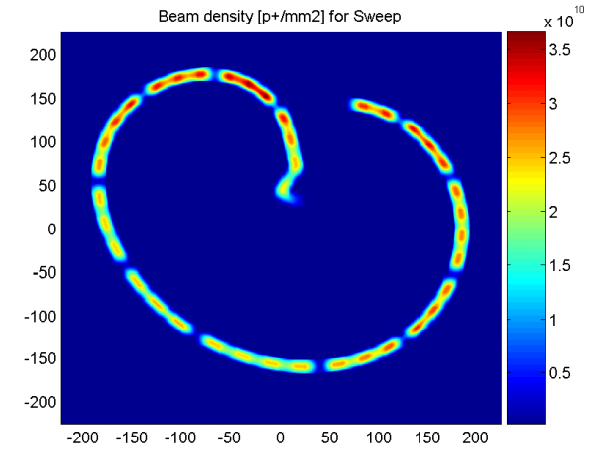
\includegraphics[width=0.5\textwidth]{figures/notes-experiment/beamdump.png}
        \item Extraction Septum magnets (MSD). Wrapped with OFHC copper (oxygen free high thermal conductivity). These magnets have a septum (gap) for the extracted beam, and a low-field hole drilled through the yoke for the circulating beam. These are preceded by a diluter block to protect them from asynchronous fire of MKD kickers. Similar treatment for quadraples. \cite{lhcDesignV1}
        \item Finally, the Beam Dump Absorber Block (TDE). Consists of carbon due to high melting temp, and thermal shock resistance. In particular, Polycrystalline Grapphite cylinders (PG) and Flexible Graphite (FG). Layout: 0.7m PG, 3.5m FG, 3.5m PG. Total 7.7m long. Cooled by water. Further sourrounded by sheilding blocks of dipole yokes filled with concrete. \cite{lhcDesignV1}
    \end{itemize}
    \item Notes about the magnets
    \begin{itemize}\scriptsize
        \item MKB and MKD field strength determined by beam energy. \cite{lhcDesignV1}
        \item MSD and MSI coils are OFHC copper, with circular cooling hole. Coated with resin epoxy. \cite{bidon}
        \item For beamdump: Horizontally deflecting kicker magnets (MKD) and vertically deflecting steel septum magnets (MSD) \cite{bidon}
        \item For injection: Vertically deflecting kicker magnets (MKD) and horizontally deflecting steel septum magnets (MSD) \cite{bidon}
    \end{itemize}
    \item Even in case of asynchronous dump (not during abort gap), no damage is expected except for quench of some magnets. There are absorbers in front of some magnets. \cite{lhcDesignV1}
\end{itemize}

\section{History of the LHC}
\begin{itemize}
    \item LHC is an interesting story
    \item Run 1 lead to the physics discoveries that motivated VH
    \item Run 1 also lead to the development of the machine that enabled Run 2
\end{itemize}
\subsection{Run 1}
This is important because of the developments and understandings that lead to Run 2. But also for discovery of Higgs
\begin{itemize}
    \item Between 2010 and 2013, energies of 3.5-4 TeV \cite{lhcRun1}
    \item Bunch structure: bunches are 150ns (2010), 75ns (2011) and 50ns (2011/2012). \cite{lhcRun1}
    \item Beams consist of bunches, grouped together in trains. \cite{lhcRun1}
    \item \textbf{2010:} \cite{lhcRun1}
    \begin{itemize}
        \item Energy 3.5 TeV \cite{lhcRun1}
        \item Commissioning run at 1.2 TeV. Physics run at 3.5 TeV. \cite{lhcRun1}
        \item First injection February 27. First collisions march 30 2010, with two bunches. \cite{lhcRun1}
        \item Over the course of months, the number of bunches, and number of particles per bunch were increased. Reached 368 bunches October 10. \cite{lhcRun1}
        \item Beam losses, caused by UFO (unidentified falling objects).  Lead to about 60 beams being dumped. \cite{lhcRun1}
        \item Unexpected oscillations in beam tune continued from 2009 to 2010. Unclear of source. Called the hump. \cite{lhcRun1}
        \item Reached bunch spacing of 50 ns towards end \cite{lhcRun1}
    \end{itemize}
    \item \textbf{2011:} \cite{lhcRun1}
    \begin{itemize}
        \item Energy 3.5 TeV \cite{lhcRun1}
        \item First beams feb 19. 3 weeks recommissioning. \cite{lhcRun1}
        \item First physics beams march 13 with 32 bunches. Ramped up to 200 bunches, 75ns bunch spacing. \cite{lhcRun1}
        \item April 21 2011 luminosity of 4.6e33 $cm^{-2}s^{-1}$, which broke hadron lumi record from Tevatron. \cite{lhcRun1}
        \item Increased bunch intensities to 1.34$\times10^{11}$ ppb. \cite{lhcRun1}
        \item The hump disappears. \cite{lhcRun1}
        \item Mean stable beam time of 6.1 hrs. 33\% efficiency for stable beams. \cite{lhcRun1}
        \item 5.6 fb$^{-1}$ provided. \cite{lhcRun1}
    \end{itemize}
    \item \textbf{2012,2013:} \cite{lhcRun1}
    \begin{itemize}
        \item Energy increased to 4 TeV to increase Higgs production cross section. \cite{lhcRun1}
        \item First stable 4 TeV beams, 3 bunches, in April 5 2012 \cite{lhcRun1}
        \item First physics beam May 4. During this time, Higgs boson was discovered. \cite{lhcRun1}
        \item Nominal scheme was 1374 bunches, 50ns spacing. Due to gaps, this means 1368 colliding bunches in ATLAS. \cite{lhcRun1}
        \item There was a plan to have private bunches colliding only in LHCb. {\color{blue}Why?} \cite{lhcRun1}
        \item Bunch intensity peaked at 1.7e11 ppb. \cite{lhcRun1}
        \item 201 days with physics collisions, 36.5\% efficient stable beams. \cite{lhcRun1}
        \item 23.3 fb$^{-1}$ provided. \cite{lhcRun1}
        \item Typical emittance is 2-2.5 microns \cite{lhcRun1}
    \end{itemize}
    \item Cryo system in run 1 was most faulty, followed by injector systems. 25-30\% of fault time. \cite{lhcRun1}
    \item Best week in run 1 was june 2012, where 1.35 fb$^{-1}$ delivered. \cite{lhcRun1}
    \item Run 1 luminosity (page 7)\\ \cite{lhcRun1}
    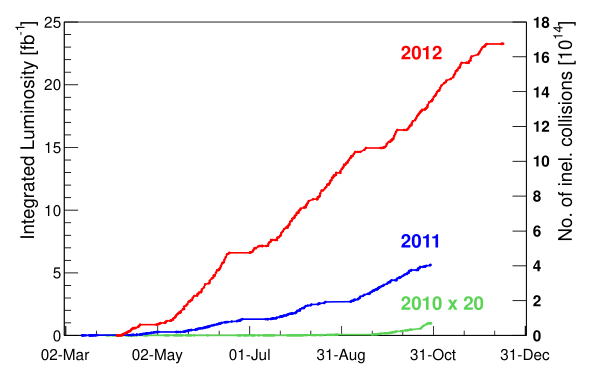
\includegraphics[width=0.8\textwidth]{figures/notes-experiment/run1Lumi.png}
    \item \textbf{Beam Cycle} (probably, should use run2 resource) \cite{lhcRun1}
    \begin{itemize}
        \item Injection. Beam is ``scraped'' by transfer line collimator's. In run 1, about 2-4\% of the beam is lost. This done in SPS. The collimator jaws heat and outgas, so these are opened as soon as injection is finished. Rings are filled consecutively (as opposed to alternating bunches) because ALICE requested it (it reduces their background??). \cite{lhcRun1}
        \item Ramp. The ramping speed is limited by dipole current ramp rate of 10 A/s, which corresponds to 6 GeV/s. A ``flat top'' of 300 s, during which the tune decay is corrected for. \cite{lhcRun1}
        \item Separation/crossing angles. {\color{red} Warning, confused} Crossing angle is 170 micro radians. Separation is on the order of mm. Horizontal separation in P1,P2. Vertical in P5,P8. Hence in IR1 beam 1 moves downward/inside. \cite{lhcRun1}
        \item Collisions. When start, tails of bunches are expelled, leading to a brief drop in expected beam lifetime. The expected lifetime of the beam is optimized by reducing the chromaticity {\color{blue} \url{https://cds.cern.ch/record/302491/files/p77.pdf}(the change in linear parameters of transverse motion with beam energy).} HOW do they reduce chromaticity? \cite{lhcRun1}
        \item Tune. The beam is large during the ramp, and reduced during squeeze. \cite{lhcRun1}
        \item Collimators. Used for squeeze, used for betatron cleaning. Used to clean ``physics debris''. \cite{lhcRun1}
    \end{itemize}
\end{itemize}

\subsection{Run 2}
\begin{itemize}
    \item Between 2015 and 2018, beam energies of 6.5 TeV and provided lumi for 160 fb$^{-1}$. \cite{lhcRun2}
    \item Peak lumi is twice design, due to small emmitance and $\beta*$ of 30 cm. \cite{lhcRun2}
    \item Combined squeeze and ramp stages \cite{lhcRun2}
    \item 25 ns bunch spacing \cite{lhcRun2}
    \item \textbf{2015} \cite{lhcRun2}
    \begin{itemize}
        \item First year of 6.5 TeV energy, with 25 ns bunch spacing. \cite{lhcRun2}
        \item First beams April 5 2015. First stable beams June 3. \cite{lhcRun2}
        \item Relaxed $\beta*=80cm$, but due to shift in the ``optical waist'' position of the beam profile, the effective $\beta*=86cm$. (This leads to a slightly lower luminosity) \cite{lhcRun2}
        \item Reached 2244 bunches by end of year. Train length is 144 bunches. \cite{lhcRun2}
        \item Intensity ramp-up limited by heat load due to e-clouds. The heating effects the cryosystems. This despite efforts to scrub. Scrubbing done with low intensity bunches. \cite{lhcRun2}
        \item Beam 2 (15R8) had a UFO storm. The beamscrean was warmed to 80 K. An obstacle was left at bottom of the chamber called ULO (Unidentified lying object). The beam was steered around ULO.ULO remained an optical for full Run 2. ULO turned out to be plastic wrapping from installation. \cite{lhcRun2}
    \end{itemize}
    \item \textbf{2016} \cite{lhcRun2}
    \begin{itemize}
        \item First beams March 25. Target $\beta*=40cm$. 25ns bunch spacing. Again, limited to 144 bunches per train. Finally reached 2220 bunches. \cite{lhcRun2}
        \item June 26, LHC reached design lumi of 1.0e34 $cm^{-2}s^{-1}$. \cite{lhcRun2}
        \item Introduced BCMS (Batch Compression Merging and Splitting), lower transverse beam size with respect to the nominal production scheme. 20\% increase in Lumi1e 1.4e34 $cm^{-2}s^{-1}$.  \cite{lhcRun2}
        \item CMS received 5-10\% higher lumi, caused by oblong beams with low vertical emittance. The crossing plane for ATLAS is vertical, while for CMS it is horizontal. \cite{lhcRun2}
        \item In August 10, short circuit in one of dipole magnets in sector 12. Decision to replace the magnet, which lead to extended shutdown. \cite{lhcRun2}
    \end{itemize}
    \item \textbf{Batch Compression Merging and Splitting}
    \begin{itemize}\scriptsize
        \item The Linac 2 beam is continuous \cite{freyermuth}
        \item The PSB has 4 rings, each of which can be overfilled by injecting the Linac 2 beam in different positions. This overfilling increases emittance. \cite{freyermuth}
        \item The ``nominal'' scheme to fill the PS from the PSB was to inject 6 bunches. Each bunch is longitudinally split into 3 bunches, then by 2, and again by 2. Total 72 bunches. \cite{freyermuth}
        \item The BCMS scheme does two things. First, 8 (instead of 6) bunches are injected to PS and spread out over two PSB cycles. This reduces the emittance in the PSB, since the required intensity is lower, and injection is spread out over fewer turns. The 8 bunches are merged to 4, then split 3x2x2. Total 48 bunches, therefore more cycles needed to fill LHC, but get higher lumi. \cite{freyermuth}
    \end{itemize}
    \item \textbf{Luminosity Anti-leveling with crossing angle}
    \begin{itemize}\scriptsize
        \item At IP beams cross at an angle. This leads to 30-40\% loss in lumi. \cite{gorzawski}
        \item The angle is set based on the intensity of the beams. Prior to 2017, the beam angle was set based on the initial intensity of the beams. Peak beam intensity \cite{gorzawski}
        \item Some lumi can be recovered by reducing the crossing angle as the beams decay.  \cite{gorzawski}
        \item A study was conducted during machine development, using standard physics setup with few bunches. \cite{gorzawski}
        \item Leveling is slow, over the course of several minutes. The adjustments for the study were in steps of 20-85 microradians. \cite{gorzawski}
        \item Corresponding TCT (Collimators jaws) move. \cite{gorzawski}
        \item Study was successful, and recommended implementation is 2017  \cite{gorzawski}
    \end{itemize}
    \item \textbf{2017} \cite{lhcRun2}
    \begin{itemize}
        \item Introduced crossing angle anti-leveling. This procedure is applied in steps of 10 microradians. Gain of 3-4\% integrated lumi per fill. {\color{blue} More info from \cite{gorzawski}} \cite{lhcRun2}
        \item 16L2 problem. Seen during commissioning were sudden losses, and large background radiation. This due to condensed air that had leaked into the magnet replacement. Tried heating the beam screen, but failed and got worse. Big drop in lumi around August. Tried to reduce the e-cloud via 8b4e cleaning sequence. This reduced the cloud, and a high-lumi version was used for physics starting in august. \cite{lhcRun2}
        \item 8b4e is 8 beam bunches, four empty buckets. \cite{lhcRun2}
        \item Higher squeeze partway through run to beta*=30cm.  \cite{lhcRun2}
        \item Lumi record set at 2.06e34 $cm^{-2}s^{-1}$. This is too high for ATLAS, so was leveled to 1.5e34 $cm^{-2}s^{-1}$ for physics. \cite{lhcRun2}
        \item 50 fb$^{-1}$ delivered \cite{lhcRun2}
    \end{itemize}
    \item \textbf{2018} \cite{lhcRun2}
    \begin{itemize}
        \item Unable to remove all water trapped in beam pipe (16L2 problem). Heating the pipe exacerbated the situation.  \cite{lhcRun2}
        \item First beam April 30 {\color{red} probably March 30, this is a mistake?}, with target beta* at 30cm, with further squeeze to 25cm.  \cite{lhcRun2}
        \item First collisions on April 17, very quick. The intensity rampup was ahead of schedule. \cite{lhcRun2}
        \item The 16L2 problem resulted in beam dumps, and was rectified by running 900 bunch beams for several hours after a dump. \cite{lhcRun2}
        \item 66 fb$^{-1}$ delivered. \cite{lhcRun2}
    \end{itemize}
    \item Run 2 history: \cite{lhcRun2}
    \item Remember the marmot! \cite{lhcRun2}
    \begin{center}
    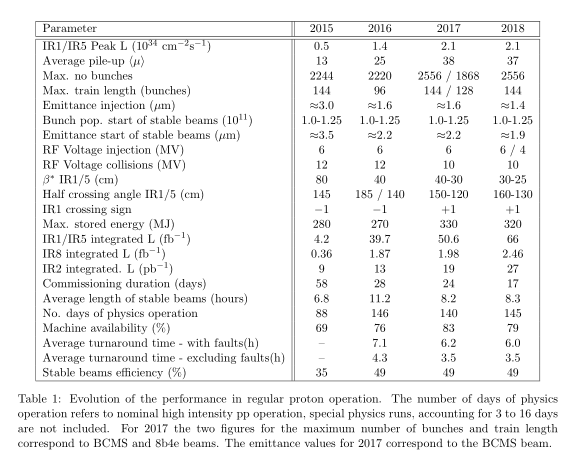
\includegraphics[width=1\textwidth]{figures/notes-experiment/run2History.png}
    \end{center}
    \item Key points from table \cite{lhcRun2}
    \begin{itemize}
        \item Lumi, pileup, bunches \cite{lhcRun2}
        \item The leveling seen in Half crossing angle \cite{lhcRun2}
        \item Stored energy \cite{lhcRun2}
        \item Commissioning days \cite{lhcRun2}
        \item Physics days \cite{lhcRun2}
        \item Stable beam efficiency \cite{lhcRun2}
    \end{itemize}
    \item \textbf{Tunes} \cite{lhcRun2}
    \begin{itemize}
        \item The tune is adjusted over the course of injection, ramp, and collisions. \cite{lhcRun2}
    \end{itemize}
    \item \textbf{Chromaticity} \cite{lhcRun2}
    \begin{itemize}
        \item Controlled to $\pm$2 units during filling. Typical values Q are +20 during filling, +15 during operation. \cite{lhcRun2}
        \item See \cite{fuchsberger} for notes on chromaticity definition \cite{lhcRun2}
    \end{itemize}
    \item \textbf{Beam optics} \cite{lhcRun2}
    \begin{itemize}
        \item Local optics corrections were often reusable from year to year, which added reliability \cite{lhcRun2}
    \end{itemize}
    \item \textbf{Emittance} \cite{lhcRun2}
    \begin{itemize}
        \item Measured by BSRT, with 10\% accuracy. \cite{lhcRun2}
        \item Stable in 2016-18 at 1.4-1.7 micrometers, which increased to 1.9um after the ramp. \cite{lhcRun2}
        \item Horizontal emittance growth due to intra-beam scattering is estimated at 0.3-0.5um/hour. Measured at 0.3-0.5 + 0.6 um/hour, additional due to e-cloud \cite{lhcRun2}
        \item Vertical emittance growth is not expected, but appears possibly due to e-cloud, is 0.3-0.6um/hour. \cite{lhcRun2}
        \item Very small emittance growth due to synchrotron radiation. \cite{lhcRun2}
    \end{itemize}
    \item \textbf{RF and bunch length} \cite{lhcRun2}
    \begin{itemize}
        \item Target bunch length 1.1ns, which decreases due to synchrotron radiation over the course of the run. It is expanded periodically. \cite{lhcRun2}
        \item Nominal RF frequency is 400,789,711 \cite{lhcRun2}
    \end{itemize}
    \item \textbf{Electron clouds} \cite{lhcRun2}
    \begin{itemize}
        \item Work was done to mitigate, but impossible to remove them \cite{lhcRun2}
        \item Causes heat load in magnets. The heat load depends on the bunch pattern, indicating the source is from e-cloud. \cite{lhcRun2}
        \item High chromaticity helped stabilize beam in presence of e-clouds. \cite{lhcRun2}
    \end{itemize}
    \item \textbf{Machine Cycle} \cite{lhcRun2}
    \begin{enumerate}
        \item \textbf{Threading} The beam was injected with low bunch intensity, stopped on collimators at each IR. The trajectory is adjusted at each step. Then several orbits are averaged to get beam position, and steering takes place. With later runs, fewer corrections needed, since beam position does not change much more than 1-2mm. \cite{lhcRun2}
        \item \textbf{Injection} SPS bunchspacing is 250ns, and reduced to 200ns over Run 2 to get more bunches in. Steering was needed, at some times for fill. Steering done only for 12-bunch trains. Most fills only have one 12-bunch train to use for steering. \cite{lhcRun2}
        \item \textbf{Ramp and squeeze} Standard ramp time is 1210s. During ramp, squeeze is normally done after reaching 2 TeV. The ramping pattern is parabolic-exponential-linear-parabolic. Squeeze continues after ramp. Adjusting the beam optics is done in steps to avoid problem tunes. \cite{lhcRun2}
        \item \textbf{Collisions} Beams are steered to collide at all interaction points. \cite{lhcRun2}
        \item \textbf{Luminosity leveling} leveled to target 1.5e34$cm^{-2}s^{-1}$ when possible. Anti-leveling by adjusting crossing angle started in 2017 in steps of 10microradians. Leveling of beta* from 30cm to 27cm to 25cm added in 2018. \cite{lhcRun2}
        \item \textbf{Beam oscillations} Observed dipolar disturbances in beams during stable beams. Earthquakes were measured from as far away as New Zealand. Tidal deformation also observed. Distortions due to mechanical resonances as well. HL-LHC civil engineering also detected due to ground compactors. \\ \cite{lhcRun2}
        \begin{center}
        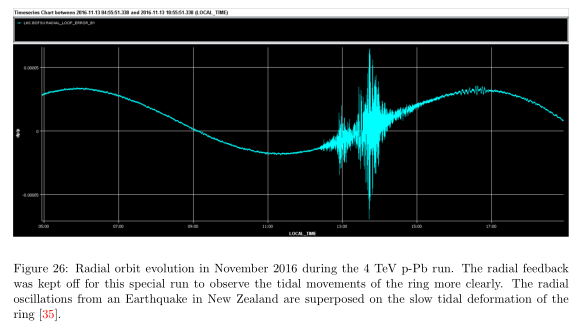
\includegraphics[width=0.6\textwidth]{figures/notes-experiment/orbit.png}
        \end{center}
    \end{enumerate}
    \item UFO rates between 1-20 per hour, but only 4 dumps caused by UFO's in 2018. Sometimes due to quenches. \cite{lhcRun2}
    \item 16L2 problem. Probably caused by frozen water introduced after magnet replacement. Heating the beampipe lead to worse problem. Bunch structure changed to 8b4e bunch structure. Before 2018, 8L of nitrogen were flushed in. This improved the situation and BCMS beams could be used. Cleaning fills were used after dumps. \cite{lhcRun2}
    \item Heavy ion history \cite{lhcRun2}
    \begin{itemize}
        \item 2015 Pb-Pb \cite{lhcRun2}
        \item 2016 Pb-p \cite{lhcRun2}
        \item 2017 Xe \cite{lhcRun2}
        \item 2018 Pb-Pb \cite{lhcRun2}
    \end{itemize}
\end{itemize}

